% Influence of the hallway width on the success of the simulation

\noi To account for the influence of the width of the hallway on the success of the simulation, we did a simulation series with different widths. The tested widths were 2.2, 2.5, 2.8, 3 and 3.5 meters. A high density flux of 1 person per second on both sides was used with a DISPERSIONFACTOR of 0.75 corresponding to a high number of overtaking attempts. The simulations were repeated with the seeds 51, 77 and 151 each. All simulations were run for 100 seconds.\\

\begin{figure}[h!]
	\centering
		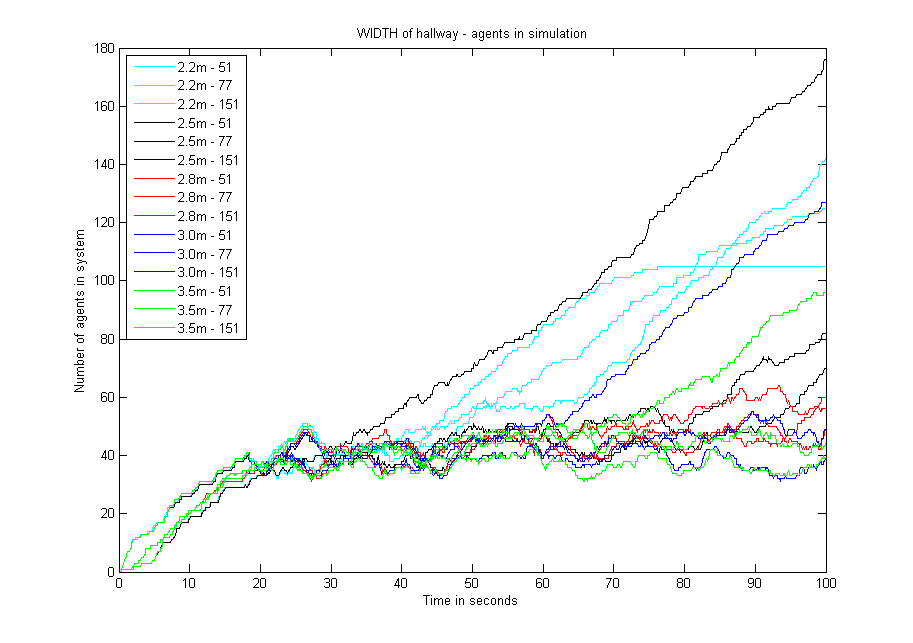
\includegraphics[width=0.80\textwidth]{../../code/sim/Width/AallInOne.png}
	\caption{The plot shows the number of agents in the system for different widths and seeds in dependence of the simulation time. This number exceeds equilibrium (around 40-50 agents) when a jam started. To show the number's dependence on the hallway width, each seed to a certain width was coloured equally. Only the hallway width was varied in these simulations. One can see here that the narrower a hallway is, the more probable jams pop up, but from 2.8 meters on it mostly worked well.}
	\label{fig:WidthAllInOne}
\end{figure}

\noi In total, 15 simulations were made. To detect jams, looking at the total number of agents in the system is an excellent way as this number starts to increase strongly when agents start to get stuck in each other. Figure \ref{fig:WidthAllInOne} shows all 15 of these numbers evolving in time. What one can clearly see is that the results are not perfect and that hazard plays a big role as eg. also a simulation of a 3.5m wide hallway got stuck, even if there was plenty of room.\\
But there are tendencies which are visible: The most obvious thing is that there really is a equilibrium the simulations are around when they work smoothly. This is where most of the graphs are. When a jam pops up, the number of agents starts to increase quite linearly because agents are spawned but can't reach the end of the hallway.\\
One can see that for 2.2m and 2.5, every simulation got stuck. Two 2.8m simulations also had a jam started at the end of the simulation. In addition to those, also a simulation of 3.0m and 3.5m each got stuck.\\

\begin{figure}[h!]
	\centering
		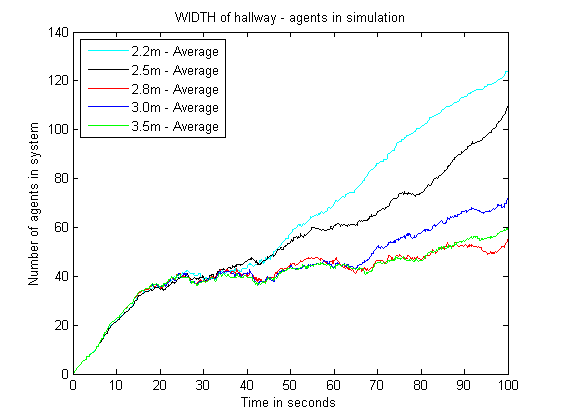
\includegraphics[width=0.80\textwidth]{../../code/sim/Width/AAveragesInOne.png}
	\caption{This plot shows the number of agents in the system for different widths and seeds in dependence of the simulation time. The numbers of three seeds were averaged to one vector for better visibility. This number exceeds equilibrium (around 40-50 agents) when a jam started. Only the hallway width was varied in these simulations. The number's dependence on the hallway width can be seen here: the narrower a hallway is, the more probable jams pop up, but from 2.8 meters on it mostly worked well. The 3.0m graph can be looked at as an exception because one of its seeds exploded quite badly, so the average looks high too.}
	\label{fig:AveragesInOne}
\end{figure}

In figure \ref{fig:AveragesInOne}, the data sets for each seeds were averaged for better visibility. One can clearly see the tendency for narrower hallways to get more jams, although the others rise up too due to the average taken over equilibrium seeds and jam seeds.\\

%Diskussion
The tendencies in this simulation series are quite obvious: The more narrow a hallway gets, the higher the probability is to get stuck, which is observed because all the 2.2m and 2.5m simulations ended in jams. Also, two of the 2.8m ended in jams, but for wider hallways, only coincidence made jams possible.\\
One can derive from this, that there is a certain width that will mostly work and is between 2.8m and 3.0m. Anything higher won't be much of an improvement because the flux is smooth but not faster. But as the hallway is narrowed, jams are inevitable.\\
